\documentclass[12pt]{article}
\usepackage{url}
\usepackage[spanish, english]{babel}
\selectlanguage{spanish}
\usepackage[fixlanguage]{babelbib}
\selectbiblanguage{spanish}
\usepackage{url}
\usepackage[utf8]{inputenc}
\usepackage{float}
\usepackage{fullpage}
\usepackage{amsmath}
\usepackage{amssymb}
\usepackage{graphicx}
\usepackage{verbatim} 
\usepackage{caption, subcaption}
\usepackage{tikz}%Generar plots
\usepackage{pgfplots}%Generar plots
\pgfplotsset{compat=1.5}
\usepackage{pgfplotstable,filecontents}
\usepackage{booktabs}
\usepackage{lipsum}

\pgfkeys{/pgf/number format/.cd,fixed,precision=5}

\usepackage[titletoc, title]{appendix}
\addto{\captionsspanish}{\renewcommand*{\appendixname}{Anexo}}

\bibliographystyle{bababbrv}

\title{Clasificación de Perros utilizando Bag of Words}
\author{Jorge Bahamonde, Sebastián González\\
\small{\url{jbahamon@ug.uchile.cl}, \url{segonzal@dcc.uchile.cl}}}
\date{}

\begin{document}
\maketitle

\section{Introducción}

La detección de animales en imágenes es una tarea compleja. La evolución ha llevado a
las criaturas a adaptarce a sus medios, siendo la mímesis con su entorno una de las claves para la supervivencia de las especies.
Los animales domésticos han evolucionado al alero de la humanidad. En tiempos modernos muchos animales viven en entornos urbanos,
y en su rol de mascotas son objetivo de retratos que son subidas a internet por sus dueños.

Presentan un problema adicional. Muchos de estos animales presentan grandes diferencias entres sus razas: tamaño, color, textura, forma, etc.
El estudio de la detección de perros en un conjunto de imágenes es un problema de interés, es un caso representativo de clasificación, para una clase con características
altamente deformables. La ventaja que brinda el estudio sobre imágenes de perros es la alta disponibilidad de imágenesde prueba en internet.
Los perros, siendo una de las mascotas más comunes, marcan una fuerte presencia en los retratos de mascotas en internet.

Se empleó la estrategia Bag of Words, una de las técnicas en el reconocimiento de patrones que arrojan mejores resultados para la clasificación.
Se puso énfasis en el estudio de esta estrategia para el reconocimiento de imágenes de perros. En particular se analizó el desempeño de la clasificación de SVM,
utilizando histogramas de palabras visuales, al variar la razón de costo asociado a los falsos positivos y falsos negativos ($\Theta$).

Se construyó un dataset de 1400 imágenes, de las cuales la mitad contienen imágenes de perros extraidas del dataset Cats and Dogs.
Las restantes imágenes no contienen perros y fueron extraidas aleatoriamente del dataset caltech-101.

\section{Descripción del Trabajo}

Se estudió el desempeño de SVM sobre histogramas de palabras visuales, siguiendo la estrategia Bag of Words.

\subsection{Generación de palabras visuales}

Se definió un corpus formado por 5000 imágenes extraidas del dataset caltech-256. Para cada imagen se calcularon los descriptores SIFT.
Estos descriptores locales fueron clusterizados utilizando k-means. Los k centroides entregados por este método se utilizaron como
palabras visuales, para la posterior clasificación.

Se generaron palabras visuales para $k = 100, 500, 1000, 1500$.

\subsection{Entrenamiento}

Se utilizó la librería libSVM, en particular el script "easy.py" incluido para entrenar cuatro modelos, cada modelo utiliza histogramas de 100, 500, 1000 ó 1500
palabras visuales. Todos los modelos fueron entrenados utilizando 500 imágenes del dataset generado.

\subsection{Clasificación}

TODO

Con los modelos entrenados, se clasificaron 400 imágenes, 200 de ellas conteniendo efectivamente perros.

Es posible modelar una característica detectando mediante un modelo estadístico sobre las características de una imágen. estas caraceteristicas vienen en forma de descriptores de palabras visuales segun la estrategia bag of words.
Usando este modelo estadistico, una imagen será clasficada como de perro si:
P de ser perro / p de ser no perro > theta

con theta un umbral.
theta puede ser descrito como la funcion de costo de tener falsos positivos y negativos.

Las distribuciones Pperro y Pnoperro son determinadas usando SVM

Explicar $\Theta$ el ratio de FPR y TPR y bla bla ROC
Esto debe servir para definir el ROC

\subsection{Dataset utilizado}
Se construyó un dataset de 1400 imágenes en total. La mitad de estas imágenes son imágenes de perros extraidas aleatoriamente del dataset Cats and Dogs. 
El resto, 700 imágenes, no contienen perros, y fueron extraidas aleatoriamente del dataset caltech-101.
Se extrajeron 500 imágenes de perros y no-perros para formar parte del set de entrenamiento.
Las 400 imágenes restantes forman el set de prueba.

\section{Resultados obtenidos}

Para evaluar el desempeño del modelo estudiado, se le ultilizó para clasificar imágenes entre dos clases:
Perro y No-Perro. Se contrastaron los resultados obtenidos con la clasificación correcta dada por la distribución en el dataset.

Se definen, en este contexto: 

\begin{itemize}
    \item el \textbf{número de positivos ($P$)} 200 imágenes en el set de prueba correspondientes a Perros.
    \item el \textbf{número de negativos ($N$)} 200 imágenes que no corresponden a Perros.
    \item el \textbf{número de falsos positivos ($FP$)} como el número de
        imágenes de prueba que el modelo identifica erroneamente como Perros.
    \item el \textbf{número de verdaderos positivos ($TP$)} como el número de
        imágenes de prueba identificadas correctamente como Perros.
    \item la \textbf{tasa de verdaderos positivos ($TPR$)} o probabilidad de detección correcta, es la razón $\frac{TP}{P}$;
    \item la \textbf{tasa de falsos positivos ($FPR$)} o probabilidad de detección incorrecta, es la razón $\frac{FP}{N}$.
\end{itemize}

De esta forma es posible estudiar el desempeño de este modelo de detección, comparando el comportamiento de ambas tasas.
El gráfico de $FPR$ versus $TPR$ al variar un tercer parámetro, en nuestro caso la función de costo $\Theta$, es denominado curva
ROC (del inglés \emph{receiver operating characteristic}).

Esta curva muestra
cuán apropiado puede ser un modelo o algoritmo para ciertas aplicaciones, ya que
el costo de un falso positivo versus un verdadero positivo varía dependiendo del
contexto.

\begin{figure}[h]
    \centering
   % \includegraphics{digit}

\begin{tikzpicture}
\begin{axis}[
        title={Curva ROC},
	xlabel={False Positive Rate},
	ylabel={True Positive Rate},
	grid=major,
	legend entries={$k=100$, $k=500$, $k=1000$, $k=1500$},
	legend style={at={(1,0)},anchor=south east},
]
\addplot table [scatter,x={FPR}, y={TPR}]{results100-ROC.csv};
\addplot table [scatter,x={FPR}, y={TPR}]{results500-ROC.csv};
\addplot table [scatter,x={FPR}, y={TPR}]{results1000-ROC.csv};
\addplot table [scatter,x={FPR}, y={TPR}]{results1500-ROC.csv};
\end{axis}
\end{tikzpicture}
    \caption{Curva ROC obtenida al variar el parámetro umbral $\Theta \in \{ 0.1,0.5,...,0.95\}$, para los cuatro modelos entrenados.}
\end{figure}

Se construyó una curva ROC a partir de los resultados de la clasificación con SVM comparando con su clasificación real conocida ya que es dada por su distribución en el dataset.

\section{Discusión}

TODO

\begin{figure}[H]
    \centering
    \subcaptionbox{No-Perro clasificado como Perro.}
{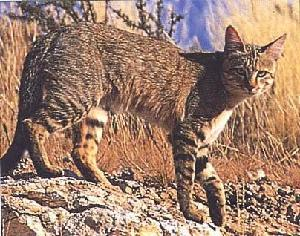
\includegraphics[scale=0.5]{../no-dogs/eval/96.jpg}}
    \subcaptionbox{Perro clasificado como No-Perro.}
{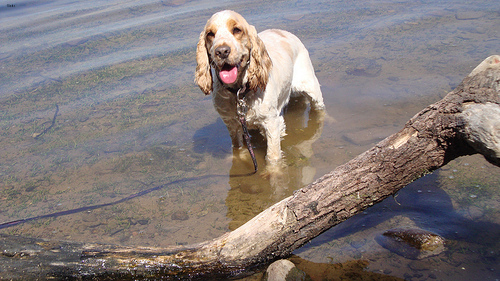
\includegraphics[scale=0.8]{../dogs/eval/14.jpg}}
    \caption{Errores de clasificación.}
\end{figure}

\section{Conclusiones}
TODO
\selectlanguage{spanish}
\selectbiblanguage{spanish}

\bibliography{./informe}

\begin{appendices}

\section{Tasas de falsos positivos y verdaderos positivos obtenidas}

\begingroup
\centering
\pgfplotstabletypeset[col sep=tab,
%     columns={theta,FPR,TPR},
     display columns/0/.style={column name=$\Theta$},
     display columns/1/.style={column name=\emph{FalsePositiveRate}},
     display columns/2/.style={column name=\emph{TruePositiveRate}},
     every head row/.style={before row=\toprule,after row=\midrule},
     every last row/.style={after row=\bottomrule},
    ]{results100-ROC.csv}
\captionof{figure}{Tasas de falsos positivos y verdaderos positivos obtenidas.}\label{fig:f}
\endgroup


\end{appendices}


\end{document} 
